\uuid{dVYA}
\exo7id{5443}
\titre{exo7 5443}
\auteur{rouget}
\organisation{exo7}
\datecreate{2010-07-10}
\isIndication{false}
\isCorrection{true}
\chapitre{Continuité, limite et étude de fonctions réelles}
\sousChapitre{Etude de fonctions}

\contenu{
\texte{
Etude complète des fonctions suivantes
}
\begin{enumerate}
    \item \question{$f_1(x)=\frac{1+x^2}{x^3}(\Arctan x-\frac{x}{1+x^2})$.}
\reponse{$f_1$ est définie et de classe $C^\infty$ sur $\Rr^*$ en vertu de théorèmes généraux. De plus, $f_1$ est paire. On étudiera $f_1$ sur $[0,+\infty[$ (se méfier alors pour la dérivabilité en $0$).

\textbf{Etude en 0} (à gauche et à droite).
\begin{align*}\ensuremath
f_1(x)&\underset{x\rightarrow0}{=}\frac{1}{x^3}(1+x^2)[x-\frac{x^3}{3}+\frac{x^5}{5}+o(x^5)-x(1-x^2+x^4+o(x^4))]\\
 &=(1+x^2)(\frac{2x^3}{3}-\frac{4x^5}{5}+o(x^5))=(1+x^2)(\frac{2}{3}-\frac{4x^2}{5}+o(x^2))\\
 &=\frac{2}{3}-\frac{2x^2}{15}+o(x^2).
\end{align*}

Par suite, $f_1$ se prolonge par continuité en $0$ en posant $f_1(0)=\frac{2}{3}$. Puisque $f_1$ admet en $0$ un développement limité d'ordre $1$, le prolongement encore noté $f_1$ est dérivable en $0$ et $f_1'(0)=0$. $C_1$ admet au point d'abscisse $0$ une tangente parallèle à $(0x)$ d'équation $y=\frac{2}{3}$. Enfin, puisque  $f(x)-\frac{2}{3}$ est, au voisinage de $0$, du signe de $-\frac{2x^2}{15}$, la courbe est localement en dessous de sa tangente.

\textbf{Etude en} $\bf{+\infty}$ (et $-\infty$). $f_1(x)\underset{x\rightarrow+\infty}{\sim}\frac{\pi}{2x}\underset{x\rightarrow+\infty}{\rightarrow}0$, et de même $f_1(x)\underset{x\rightarrow-\infty}{\rightarrow}0$.

\textbf{Dérivée, variations.}

Pour $x>0$, 

\begin{align*}\ensuremath
f'(x)&=(-\frac{3}{x^4}-\frac{1}{x^2})
(\Arctan x-\frac{x}{1+x^2})+\frac{1+x^2}{x^3}(\frac{1}{1+x^2}-\frac{1-x^2}{(1+x^2)^2})\\
 &=-\frac{3+x^2}{x^4}(\Arctan x-\frac{x}{1+x^2})+\frac{1+x^2}{x^3}\frac{2x^2}{(1+x^2)^2}\\
 &=\frac{3+x^2}{x^4}(-\Arctan x+\frac{x}{1+x^2}+\frac{x^4}{3+x^2}\frac{2}{x(1+x^2)})\\
 &=\frac{3+x^2}{x^4}(-\Arctan x+\frac{x(3+x^2)+2x^3}{(1+x^2)(3+x^2))}=\frac{3+x^2}{x^4}g(x)
\end{align*}

où, pour tout réel $x$, $g(x)=-\Arctan x+\frac{3x}{3+x^2}$.

$g$ est dérivable sur $\Rr$ et pour $x$ réel,

$$g'(x)=3\frac{(3+x^2)-2x^2}{(3+x^2)^2}-\frac{1+x^2}=\frac{3(3-x^2)(1+x^2)-(3+x^2)^2}{(1+x^2)(3+x^2)^2}=\frac{-4x^4}{(3+x^2)^2(1+x^2)}.$$

$g'$ est donc strictement négative sur $]0,+\infty[$ et par suite, $g$ est donc strictement décroisante sur $[0,+\infty[$. Puisque $g(0)=0$, pour $x>0$, $g(x)<0$. Finalement, $f_1'$ est strictement négative sur $]0,+\infty[$ et $f_1$ est strictement décroissante sur $[0,+\infty[$.

Le tableau de variations de $f_1$ n'apporte rien de plus.

\textbf{Graphe}

$$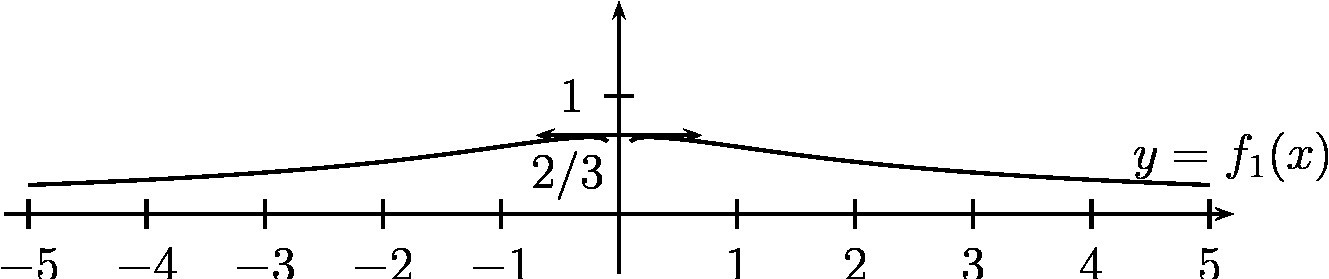
\includegraphics{../images/img005443-4}$$

%%%%%%%%%%%%%%%%%%%%%%%%%%%%%%%%%%%%%%%%%%%%%%%%%%%%%%%%%%%%%%%%%%%%%%%%%%%%%%%%%%%%%%%%%%%%%%%%%%%%%%%%%%%%%%%%%%%%%}
    \item \question{$f_2(x)=|\tan x|+\cos x$.}
\reponse{$f_2$ est définie sur $D=\Rr\setminus(\frac{\pi}{2}+\pi\Zz)$, paire et $2\pi$-périodique. $f_2$ est continue sur $D$ en vertu de théorèmes généraux. On étudie $f_2$ sur $[0,\frac{\pi}{2}[\cup]\frac{\pi}{2},\pi]$.

\textbf{Etude en} $\bf{\frac{{\pi}}{2}}$.

$f(x)\underset{x\rightarrow\pi/2}{\sim}|\tan x|$ et donc, $\lim_{x\rightarrow \pi/2}f(x)=+\infty$. $C_2$ admet la droite d'équation $x=\frac{\pi}{2}$ pour droite asymptote.

\textbf{Dérivabilité et dérivée.}

$f_2$ est dérivable sur $\Rr\setminus\frac{\pi}{2}\Zz$ en vertu de théorèmes généraux et pour $x\notin\frac{\pi}{2}\Zz$, $f_2'(x)=\varepsilon\frac{1}{\cos^2x}-\sin x$ où $\varepsilon$ est le signe de $\tan x$.

$f_2$ est aussi dérivable à droite en $0$ et $(f_2)_d'(0)=1$. Par symétrie, $f_2$ est dérivable à gauche en $0$ et $(f_2)_g'(0)=-1$. $f_2$ n'est pas dérivable en $0$.

De même, $f_2$ est dérivable à gauche et à droite en $\pi$ avec $(f_2)_g'(\pi)=-1$ et $(f_2)_d'(\pi)=1$, et n'est donc pas dérivable en $\pi$.

\textbf{Variations}.

$f_2$ est strictement décroissante sur $]\frac{\pi}{2},\pi]$ en tant que somme de deux fonctions strictement décroissantes sur $]\frac{\pi}{2},\pi]$. Puis, pour $x$ élément de $]0,\frac{\pi}{2}[$, $f_2'(x)=\frac{1}{\cos^2x}-\sin x>1-1=0$. $f_2'$ est strictement positive sur $]0,\frac{\pi}{2}[$ et donc $f_2$ est strictement croissante sur $[0,\frac{\pi}{2}[$.

\textbf{Graphe.}

$$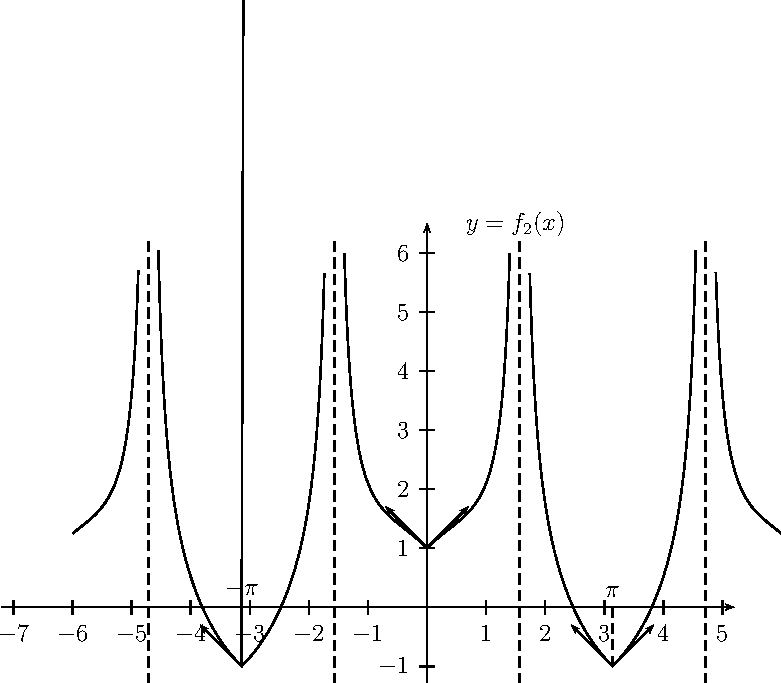
\includegraphics{../images/img005443-5}$$

%%%%%%%%%%%%%%%%%%%%%%%%%%%%%%%%%%%%%%%%%%%%%%%%%%%%%%%%%%%%%%%%%%%%%%%%%%%%%%%%%%%%%%%%%%%%%%%%%%%%%%%%%%%%%%%%%%%%}
    \item \question{$f_3(x)=x-\ln\left|\frac{120+60x+12x^2+x^3}{120-60x+12x^2-x^3}\right|$.}
\reponse{Pour $x$ réel, posons $P(x)=x^3+12x^2+60x+120$. Pour tout réel $x$, on a $P'(x)=3(x^2+8x+20)=3((x+4)^2+4)>0$. $P$ est une fonction polynôme de degré $3$ strictement croissante sur $\Rr$ et s'annule donc une et une seule fois en un certain réel noté $\alpha$. De plus, $P(-5)P(-4)<0$ et $\alpha\in]-5,-4[$.

Enfin, $P$ est strictement négatif sur $]-\infty,\alpha[$ et strictement positif sur $]\alpha,+\infty[$.

$f_3$ est définie sur $\Rr\setminus\{-\alpha,\alpha\}$, et pour $x\in\Rr\setminus\{-\alpha,\alpha\}$, 

$$f_3(x)=x-\ln\left|\frac{P(x)}{P(-x)}\right|=x-\ln|P(x)|+\ln|P(-x)|.$$
 
Notons que $f_3$ est impaire.
 
\textbf{Dérivabilité et dérivée.}

$f_3$ est de classe $C^\infty$ sur $\Rr\setminus\{-\alpha,\alpha\}$ en vertu de théorèmes généraux et pour $x\in\Rr\setminus\{-\alpha,\alpha\}$,

$$f_3'(x)=1-\frac{P'(x)}{P(x)}-\frac{P'(-x)}{P(-x)}=\frac{P(x)P(-x)-P'(x)P(-x)-P'(-x)P(x)}{P(-x)P(x)}.$$

Puis,

\begin{align*}\ensuremath 
P(x)P(-x)&-P'(x)P(-x)-P'(-x)P(x)\\
 &=((12x^2+120)+(x^3+60x))((12x^2+120)-(x^3+60x))\\
 &\;-3((x^2+20)+8x)((12x^2+120)-(x^3+60x)))-
3((x^2+20)-8x))((12x^2+120)+(x^3+60x))\\
 &=144(x^2+10)^2-x^2(x^2+60)^2-6((x^2+20)(12x^2+120)-(8x)(x^3+60x))\\
 &=(-x^6+24x^4-720x^2+14400)-6(4x^4-120x^2+2400)=-x^6,
\end{align*}

et donc $f_3'(x)=\frac{-x^6}{P(x)P(-x)}$.

\textbf{Etude en} $\bf{+{\infty}}$.

$$f_3(x)-x\underset{x\rightarrow+\infty}{=}-\ln(1+\frac{12}{x}+o(\frac{1}{x}))+\ln(1-\frac{12}{x}+o(\frac{1}{x}))=-\frac{24}{x}+o(\frac{1}{x}).$$

On en déduit tout d'abord que $\lim_{x\rightarrow +\infty}f_3(x)=+\infty$ (resp.$\lim_{x\rightarrow -\infty}f_3(x)=-\infty$, puis que $C_3$ admet en $+\infty$ (resp.$-\infty$) la droite d'équation $y=x$ pour droite asymptote et que $C_3$ est au-dessous (resp. au-dessus) de cette droite au voisinage de $+\infty$ (resp.$-\infty$).

\textbf{Variations.}

D'une part, $f_3'(0)=0$. D'autre part, pour $x>0$, $P(x)>0$. $f_3'$ est donc du signe de $-P(-x)$ sur $]0,+\infty[\setminus\{\alpha\}$. Ainsi, $f_3'$ est strictement négative sur $]0,\alpha[$ et strictement positive sur $]\alpha,+\infty[$.

On en déduit le tableau de variations de $f_3$.


$$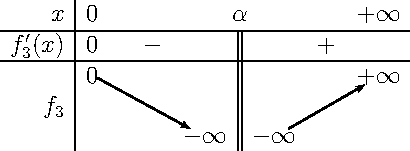
\includegraphics{../images/img005443-1}$$


\textbf{Graphe}.

$$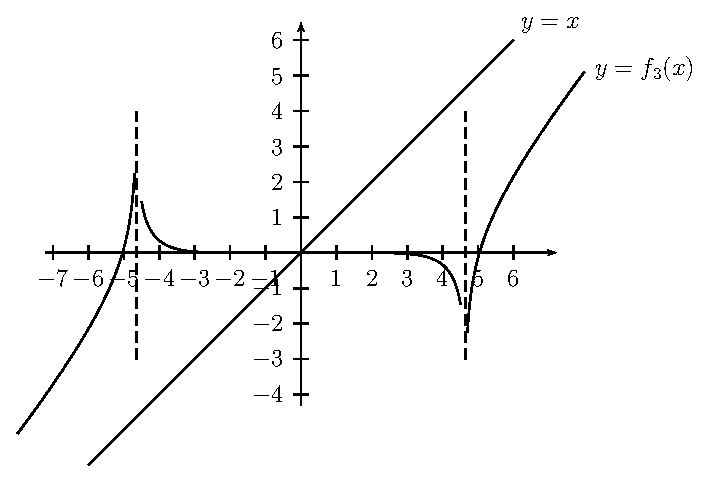
\includegraphics{../images/img005443-6}$$


%%%%%%%%%%%%%%%%%%%%%%%%%%%%%%%%%%%%%%%%%%%%%%%%%%%%%%%%%%%%%%%%%%%%%%%%%%%%%%%%%%%%%%%%%%%%%%%%%%%%%%%%%%%%%%%%%%%%%%}
    \item \question{$4_(x)=xe^{\frac{2x}{x^2-1}}$.}
\reponse{$f_4$ est définie sur $\Rr\setminus\{-1,1\}$. De plus, pour $x\neq 0$, 

$$f_4(\frac{1}{x})=\frac{1}{x}e^{\frac{2/x}{1/x^2-1}}=\frac{1}{x}e^{-\frac{2x}{x^2-1}}=\frac{1}{f_4(x)}.$$

Ce genre de constatation peut servir à calculer $\lim_{x\rightarrow +\infty}f_4(x)$ si l'on connait $\lim_{x\rightarrow 0,\;x>0}f_4(x)$, obtenir les variations de $f_4$ sur $]0,1[$ si on les connait sur $]1,+\infty[$ ...

On peut aussi noter que $\forall x\in\Rr\setminus\{-1,1\}$, $f_4(-x)f_4(x)=-x^2$ et donc, pour $x\neq 0$, $f_4(-x)=\frac{-x^2}{f_4(x)}$. Cette constatation pourra être utile pour déduire l'étude de $f_4$ en $-1$ de l'étude en $1$.

\textbf{Etude en} $\bf{+{\infty}}$ \textbf{et} $\bf{-{\infty}}$.

Puisque $\frac{2x}{x^2-1}\underset{x\rightarrow\pm\infty}{\rightarrow}0$, on a  $f_4(x)\underset{x\rightarrow\pm\infty}{\sim}x$ ce qui montre déjà que $\lim_{x\rightarrow +\infty}f_4(x)=+\infty$, $\lim_{x\rightarrow -\infty}f_4(x)=-\infty$ et que $C_4$ admet en $+\infty$ et $-\infty$, une direction asymptotique d'équation $y=x$. Plus précisément,

$$\frac{2x}{x^2-1}\underset{x\rightarrow\pm\infty}{=}\frac{2}{x}(1-\frac{1}{x^2})^{-1}=\frac{2}{x}+o(\frac{1}{x^2}),$$

puis,

$$e^{\frac{2x}{x^2-1}}\underset{x\rightarrow\pm\infty}{=}1+(\frac{2}{x})+(\frac{2}{x})^2+ o(\frac{1}{x^2})=1+\frac{2}{x}+\frac{2}{x^2}+ o(\frac{1}{x^2}).$$

On en déduit que

$$f_4(x)\underset{x\rightarrow\pm\infty}{=}x+2+\frac{2}{x}+o(\frac{1}{x}).$$

Par suite, $C_4$ admet la droite d'équation $y=x+2$ pour droite asymptote en $+\infty$ et $-\infty$. De plus, le signe de $f_4(x)-(x+2)$ étant localement le signe de $\frac{2}{x}$, $C_4$ est au-dessus de son asymptote au voisinage de $+\infty$ et au-dessous au voisinage de $-\infty$.

\textbf{Etude en 1 (et -1).}

Clairement, $\lim_{x\rightarrow 1,\;x>1}f_4(x)=+\infty$ et $\lim_{x\rightarrow -1,\;x>-1}f_4(x)=-\infty$. Ensuite, $\lim_{x\rightarrow 1,\;x<1}f_4(x)=0$ et $\lim_{x\rightarrow -1,\;x<-1}f_4(x)=0$.

On prolonge $f_4$ par continuité à gauche en $1$ en posant $f_4(1)=0$, et de même en $-1$ et on étudie la dérivabilité du prolongement encore noté $f_4$.

$f_4$ est continue sur $]-1,1]$, de classe $C^1$ sur $]-1,1[$ et pour $x\in]-1,1[$ (voir dérivée-variations), 

$$f_4'(x)=\frac{x^4-2x^3-2x^2-2x+1}{(x^2-1)^2}e^{\frac{2x}{x^2-1}}\underset{x\rightarrow1,\;x<1}{\rightarrow}0.$$

D'après un théorème classique d'analyse, $f_4$ est de classe $C^1$ sur $]-1,1]$ et en particulier dérivable à gauche en $1$ et $f_g'(1)=0$.

De même, $f_4$ est dérivable à gauche en $-1$ et $f_g'(-1)=0$. $C_4$ admet en ces points des demi-tangentes parallèles à l'axe $(Ox)$.

\textbf{Dérivée. Variations.}

$f_4$ est de classe $C^1$ sur $\Rr\setminus\{-1,1\}$ en vertu de théorèmes généraux et pour $x\neq 0$,

\begin{align*}\ensuremath
\frac{f_4'(x)}{f_4(x)}&=(\ln|f_4|)'(x)=(\ln|x|+\frac{2x}{x^2-1})'(x)=\frac{1}{x}+2\frac{(x^2-1)-x(2x)}{(x^2-1)^2}\\
 &=\frac{(x^2-1)^2-2x(x^2+1)}{x(x^2-1)^2}=\frac{x^4-2x^3-2x^2-2x+1}{x(x^2-1)^2},
\end{align*}
 
et donc 

$$\forall x\neq 0,\;f4'(x)=\frac{x^4-2x^3-2x^2-2x+1}{(x^2-1)^2}e^{\frac{2x}{x^2-1}},$$

ce qui reste vrai pour $x=0$ par continuité de $f_4'$ en $0$.

$f_4'$ est donc du signe de $P(x)=x^4-2x^3-2x^2-2x+1$. Or, pour $x\neq0$,

\begin{align*}\ensuremath 
P(x)&=x^2((x^2+\frac{1}{x^2})-2(x+\frac{1}{x})-2)=x^2((x+\frac{1}{x})^2-2(x+\frac{1}{x})-4)=\\
 &=x^2(x+\frac{1}{x}-(1-\sqrt{5})(x+\frac{1}{x}-(1+\sqrt{5}))=(x^2-(1-\sqrt{5})x+1)(x^2-(1+\sqrt{5})x+1),
\end{align*}

ce qui reste vrai pour $x=0$.

Le premier trinôme a un discriminant égal à $(\sqrt{5}-1)^2-4=2-2\sqrt{5}<0$ et donc $\forall x\in\Rr,\;x^2-(1-\sqrt{5})x+1>0$.

Le deuxième trinôme a un discriminant égal à $(\sqrt{5}+1)^2-4=2+2\sqrt{5}>0$ et admet donc deux racines réelles $\alpha=\frac{1}{2}(1+\sqrt{5}+\sqrt{2+\sqrt{5}})2,89...>1$ et $\beta=\frac{1}{2}(1+\sqrt{5}-\sqrt{2+2\sqrt{5}})=\frac{1}{\alpha}0,34...\in]0,1[$.
On en déduit le tableau de variation de $f_4$.

$$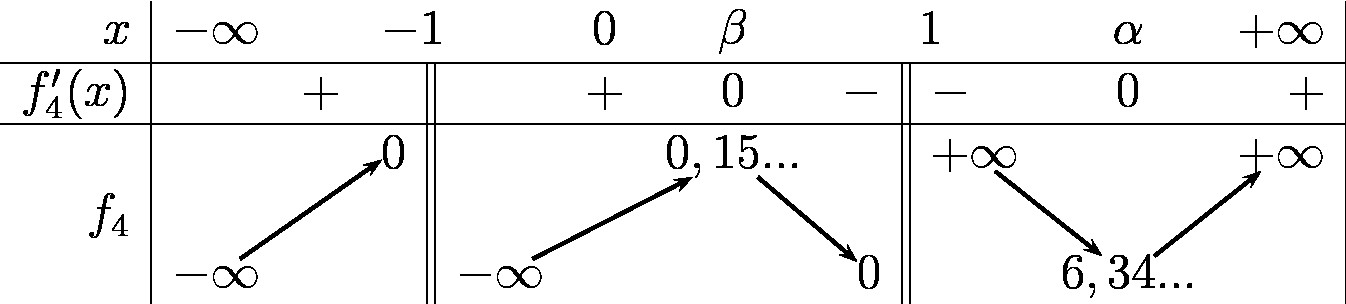
\includegraphics{../images/img005443-2}$$

\textbf{Graphe.}

$$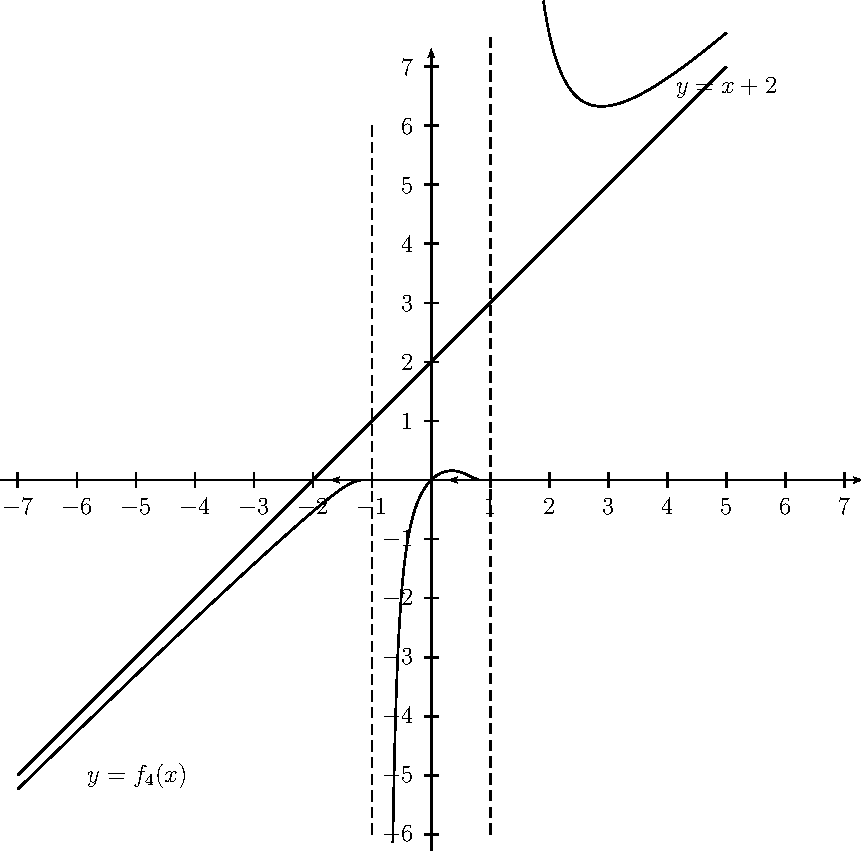
\includegraphics{../images/img005443-7}$$


%%%%%%%%%%%%%%%%%%%%%%%%%%%%%%%%%%%%%%%%%%%%%%%%%%%%%%%%%%%%%%%%%%%%%%%%%%%%%%%%%%%%%%%%%%%%%%%%%%%%%%%%%%%%%%%%}
    \item \question{$f_5(x)=\frac{1}{x}\ln\left(\frac{e^x-1}{x}\right)$.}
\reponse{Si $x>0$, $e^x-1>0$ et si $x<0$, $e^x-1<0$. Donc, pour $x\neq 0$, $ > 0$ et $f_5$ est définie sur $\Rr^*$.
Pour $x\neq 0$, 

$$f_5(-x)=-\frac{1}{x}\ln\frac{e^{-x}-1}{-x}=-\frac{1}{x}\ln(e^{-x})-\frac{1}{x}\ln\frac{e^x-1}{x}=1-f(x).$$

Donc, pour tout réel non nul $x$, $f(x)+f(-x)=1$. Le point de coordonnées $(0,\frac{1}{2})$ est centre de 
symétrie de $C_5$.

\textbf{Etude en 0.}

$$f_5(x)\underset{x\rightarrow0}{=}\frac{1}{x}\ln(1+\frac{x}{2}+\frac{x^2}{6}+o(x^2))=\frac{1}{x}((\frac{x}{2}+\frac{x^2}{6})-\frac{1}{2}(\frac{x}{2})^2+o(x^2))=\frac{1}{2}+\frac{1}{24}x+o(x).$$

Ainsi, $f_5$ se prolonge par continuité en $0$ en posant $f_5(0)=\frac{1}{2}$. Le prolongement, encore noté $f_5$, admet en $0$ un développement limité d'ordre $1$ et est donc dérivable en $0$ avec $f_5'(0)=\frac{1}{24}$. Une équation de la tangente à $C_5$ en le point d'abscisse $0$ est $y=\frac{1}{24}x+\frac{1}{2}$. Par symétrie, ce point est un point d'inflexion.

\textbf{Etude en} $\bf{+{\infty}}$.

$$f_5(x)\underset{x\rightarrow+\infty}{=}\frac{1}{x}(\ln(e^x)+\ln(1-e^{-x})-\ln x)=1-\frac{\ln x}{x}+\frac{\ln(1-e^{-x}}{x}=1+o(1).$$

Donc, $\lim_{x\rightarrow +\infty}f_5(x)=1$. Par symétrie, $\lim_{x\rightarrow -\infty}f_5(x)=\lim_{x\rightarrow -\infty}(1-f_5(-x))=1-1=0$.

\textbf{Dérivée. Variations.}

$f_5$ est dérivable sur $\Rr^*$ en vertu de théorèmes généraux (et donc sur $\Rr$) et pour $x\neq 0$, (puisque $\ln\frac{e^x-1}{x}=\ln\left|\frac{e^x-1}{x}\right|=\ln|e^x-1|-\ln|x|$),

$$f_5'(x)=-\frac{1}{x^2}\ln\frac{e^x-1}{x}+\frac{1}{x}(\frac{e^x}{e^x-1}-\frac{1}{x})
=\frac{1}{x^2}(-\ln\frac{e^x-1}{x}+\frac{xe^x}{e^x-1}-1).$$

$f_5'$ est, sur $\Rr^*$, du signe de $g(x)=-\ln\frac{e^x-1}{x}+\frac{xe^x}{e^x-1}+-1$. $g$ est dérivable sur $\Rr^*$ et pour $x$ réel non nul,

\begin{align*}\ensuremath
g'(x)&=-\frac{e^x}{e^x-1}+\frac{1}{x}+\frac{(e^x+xe^x)(e^x-1)-xe^x.e^x}{(e^x-1)^2}
=\frac{-xe^x(e^x-1)+(e^x-1)^2+xe^x(e^x-x-1)}{x(e^x-1)^2}\\
 &=\frac{(e^x-1)^2-x^2e^x}{x(e^x-1)^2}=\frac{(e^{x/2}-e^{-x/2})^2-x^2}{x(e^{x/2}-e^{-x/2})^2}\\
 &=\frac{(2\sh\frac{x}{2})^2-x^2}{x(2\sh\frac{x}{2})^2}=\frac{\sh^2\frac{x}{2}-(\frac{x}{2})^2}{x\sh^2\frac{x}{2}}.
\end{align*} 
 
L'inégalité $\sh x>x$, valable pour $x>0$, est classique (par exemple, la formule de \textsc{Taylor}-\textsc{Laplace} à l'ordre 1 fournit pour $x>0$, $\sh x=x+\int_{0}^{x}(x-t)\sh t\;dt>x$.) Par suite, $g'$ est strictement positive sur $]0,+\infty[$, et donc $g$ est strictement croissante sur $]0,+\infty[$. En tenant compte de $g(0^+)= 0$, $g$ est donc strictement positive sur $]0,+\infty[$. Il en est de même de $f_5'$ et $f_5$ est strictement croissante sur $]0,+\infty[$.

Par symétrie et continuité en $0$, $f_5$ est strictement croissante sur $\Rr$.

\textbf{Graphe.}

$$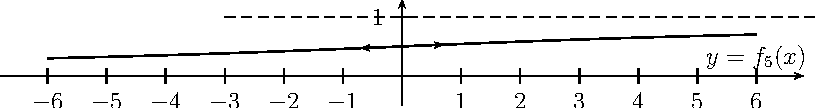
\includegraphics{../images/img005443-8}$$


%%%%%%%%%%%%%%%%%%%%%%%%%%%%%%%%%%%%%%%%%%%%%%%%%%%%%%%%%%%%%%%%%%%%%%%%%%%%%%%%%%%%%%%%%%%%%%%%%%%%%%%%%%%%%%%%%%%%%}
    \item \question{$f_6(x)=x+\sqrt{|x^2-1|}$.}
\reponse{$f_6$ est définie et continue sur $\Rr$, dérivable sur $\Rr\{-1,1\}$ en vertu de théorèmes généraux.

\textbf{Etude en 1.}

$f_6(x)-f_6(1)=x-1+\sqrt{|x^2-1|}\underset{x\rightarrow1}{\sim}\sqrt{2}\sqrt{|x-1|}$, ce qui montre que $f_6$ n'est pas dérivable en $1$ mais que $C_6$ admet au point d'abscisse $1$ deux demi-tangentes parallèles à $(Oy)$.

\textbf{Etude en -1.}

$f_6(x)-f_6(-1)=x+1+\sqrt{|x^2-1|}\underset{x\rightarrow-1}{\sim}\sqrt{2}\sqrt{|x+1|}$,  ce qui montre que $f_6$ n'est pas dérivable en $-1$ mais que $C_6$ admet au point d'abscisse $-1$ deux demi-tangentes parallèles à $(Oy)$.

\textbf{Etude en} $\bf{+{\infty}}$.

Au voisinage de $+\infty$, on a

$$f_6(x)=x+x(1-\frac{1}{x^2})^{1/2}=x+x(1-\frac{1}{2x^2}+o(\frac{1}{x^2}))=2x-\frac{1}{2x}+o(\frac{1}{x}),$$

ce qui montre tout à la fois que $\lim_{x\rightarrow +\infty}f_6(x)=+\infty$, puis que la droite d'équation $y=2x$ est asymptote à $C_6$ en $+\infty$ et que $C_6$ est au-dessous de cette droite au voisinage de $+\infty$.

\textbf{Etude en} $\bf{-{\infty}}$.

Au voisinage de $-\infty$, on a, $f_6(x)=x-x(1+o(\frac{1}{x}))=o(1)$, et $\lim_{x\rightarrow -\infty}f_6(x)=0$.

\textbf{Dérivée. Variations.}

Soit $\varepsilon$ le signe de $x^2-1$. Pour $x\neq\pm1$, 

$$f_6'(x)=1+\frac{2\varepsilon x}{2\sqrt{\varepsilon(x^2-1)}}=\frac{\sqrt{\varepsilon(x^2-1)}+\varepsilon x}{\sqrt{\varepsilon(x^2-1)}}.$$

Si $-1<x\leq0$, (de sorte que $\varepsilon x>0$) ou $x>1$, $f_6'(x)>0$.

Si $x<-1$, $\mbox{sgn}(f_6'(x))=\mbox{sgn}(x+\sqrt{x^2-1})=\mbox{sgn}(\frac{1}{x-\sqrt{x^2-1}}=-$ et $f_6'(x)<0$.

Si $0\leq x<1$. $\mbox{sgn}(f_6'(x))=\mbox{sgn}(-x+\sqrt{x^2-1})=\mbox{sgn}(-x^2-(x^2-1))=\mbox{sgn}(\frac{1}{\sqrt{2}}-x)$.

D'où le tableau de variations de $f_6$~:

$$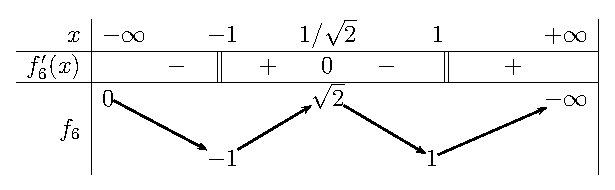
\includegraphics{../images/img005443-3}$$



\textbf{Graphe.}

$$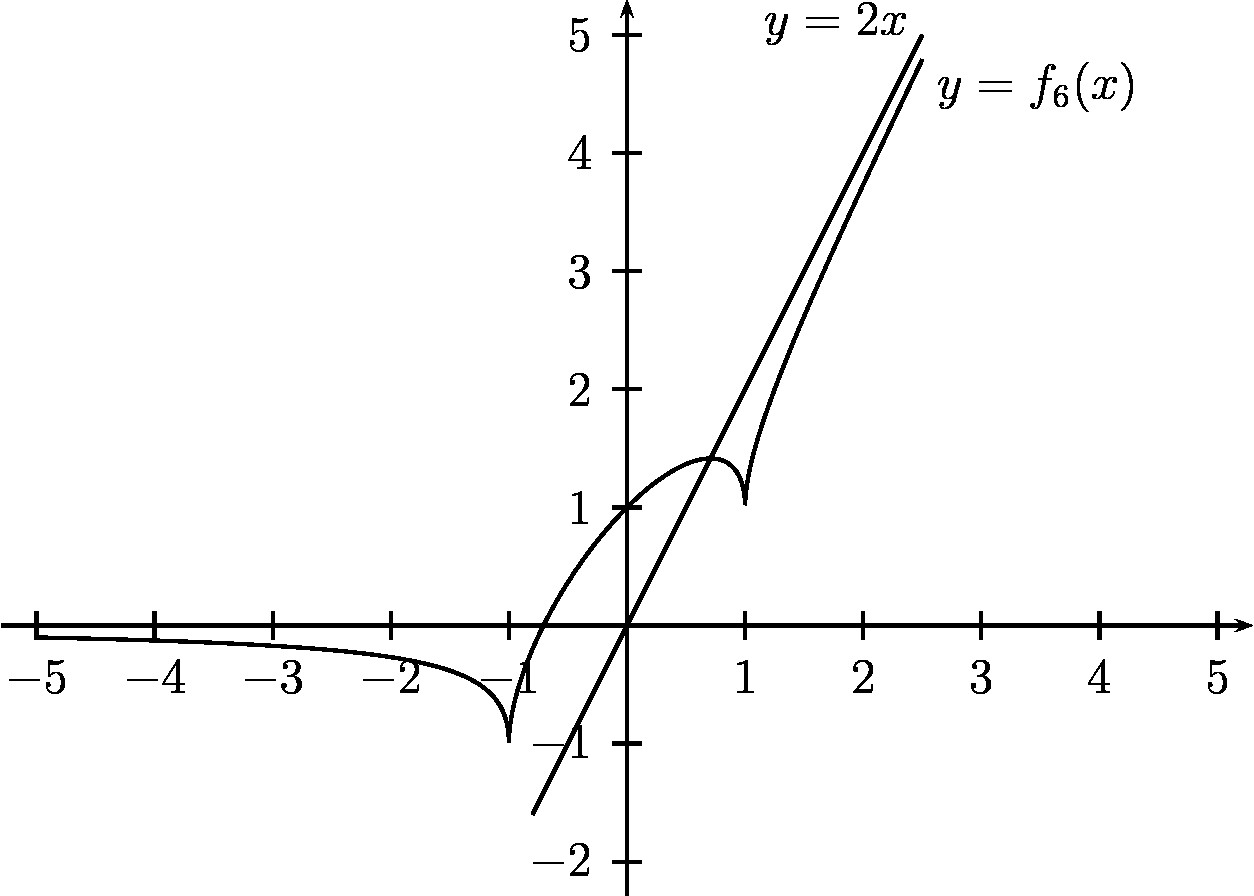
\includegraphics{../images/img005443-9}$$



%%%%%%%%%%%%%%%%%%%%%%%%%%%%%%%%%%%%%%%%%%%%%%%%%%%%%%%%%%%%%%%%%%%%%%%%%%%%%%%%%%%%%%%%%%%%%%%%%%%%%%%%%%%%%%%%%%%%%}
    \item \question{$f_7(x)=e^{/\ln x}$.}
\reponse{$$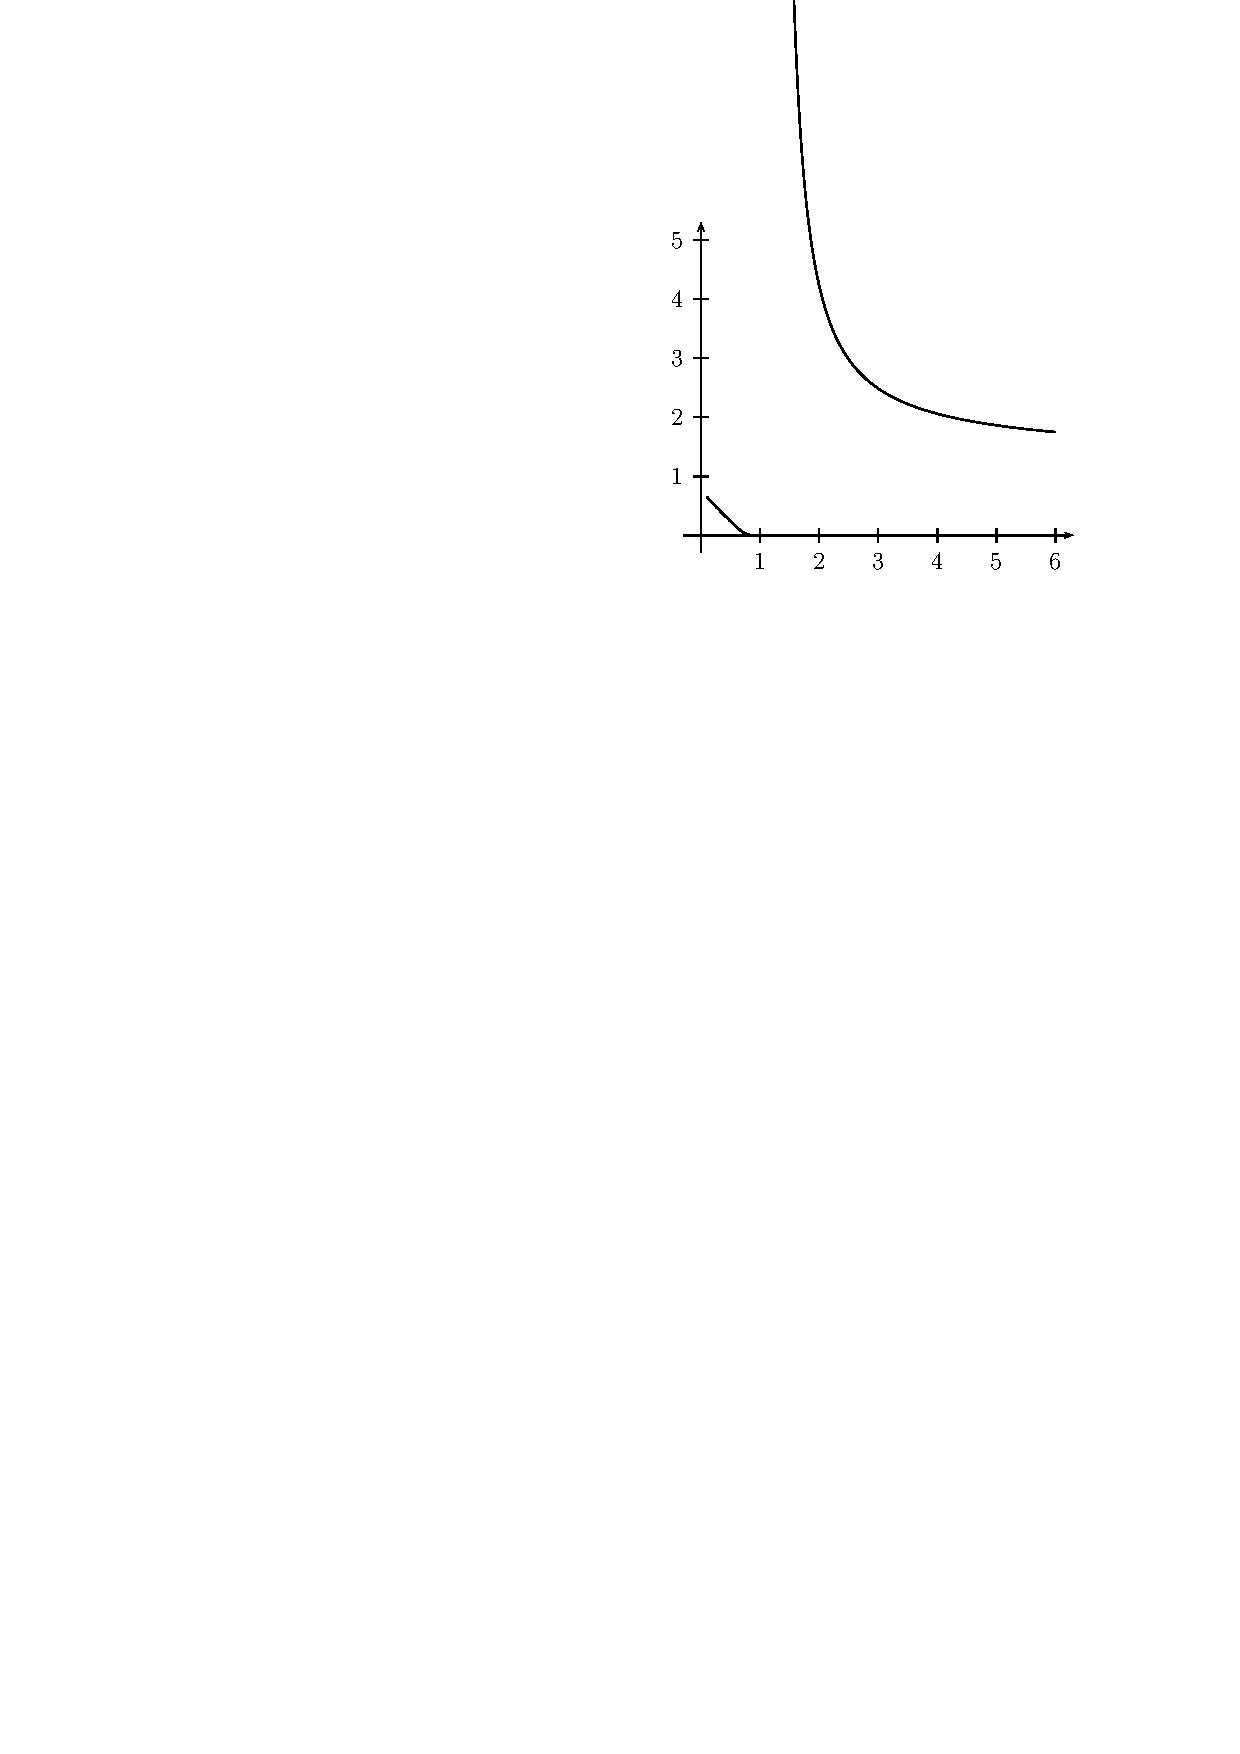
\includegraphics{../images/img005443-10}$$


%%%%%%%%%%%%%%%%%%%%%%%%%%%%%%%%%%%%%%%%%%%%%%%%%%%%%%%%%%%%%%%%%%%%%%%%%%%%%%%%%%%%%%%%%%%%%%%%%%%%%%%%%%%%%%%%%%%%%}
    \item \question{$f_8(x)=\left(1+\frac{1}{x}\right)^x$.}
\reponse{%%%%%%%%%%%%%%%%%%%%%%%%%%%%%%%%%%%%%%%%%%%%%%%%%%%%%%%%%%%%%%%%%%%%%%%%%%%%%%%%%%%%%%%%%%%%%%%%%%%%%%%%%%%%%%%%%%%%%}
    \item \question{$f_9(x)=\mbox{log}_2(1-\mbox{log}_{\frac{1}{2}}(x^2-5x+6))$.}
\reponse{%%%%%%%%%%%%%%%%%%%%%%%%%%%%%%%%%%%%%%%%%%%%%%%%%%%%%%%%%%%%%%%%%%%%%%%%%%%%%%%%%%%%%%%%%%%%%%%%%%%%%%%%%%%%%%%%%%%%%}
    \item \question{$f_{10}(x)=E(x)+(x-E(x))^2$.}
\reponse{$$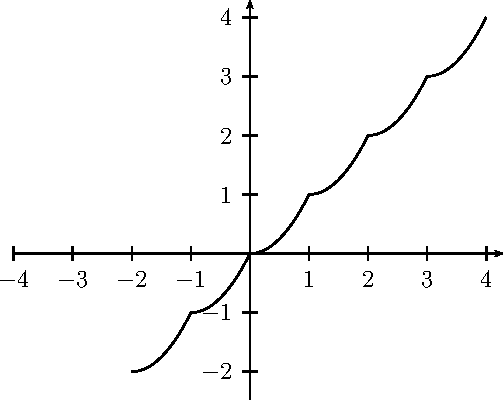
\includegraphics{../images/img005443-11}$$


%%%%%%%%%%%%%%%%%%%%%%%%%%%%%%%%%%%%%%%%%%%%%%%%%%%%%%%%%%%%%%%%%%%%%%%%%%%%%%%%%%%%%%%%%%%%%%%%%%%%%%%%%%%%%%%%%%%%%}
    \item \question{$f_{11}(x)=\Arcsin\sqrt{\frac{1}{2}-x}+\Arcsin\sqrt{\frac{1}{2}+x}$.}
\reponse{$$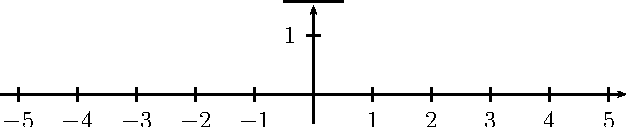
\includegraphics{../images/img005443-12}$$


%%%%%%%%%%%%%%%%%%%%%%%%%%%%%%%%%%%%%%%%%%%%%%%%%%%%%%%%%%%%%%%%%%%%%%%%%%%%%%%%%%%%%%%%%%%%%%%%%%%%%%%%%%%%%%%%%%%%%}
    \item \question{$f_{12}(x)=\frac{\Arcsin x}{x}$.}
\reponse{$$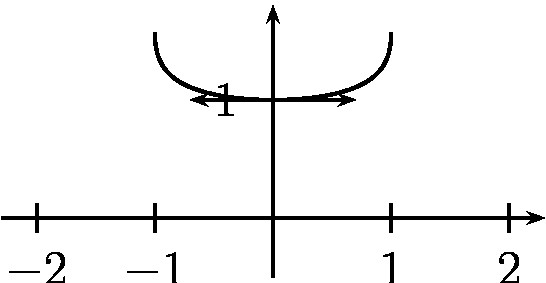
\includegraphics{../images/img005443-13}$$



%%%%%%%%%%%%%%%%%%%%%%%%%%%%%%%%%%%%%%%%%%%%%%%%%%%%%%%%%%%%%%%%%%%%%%%%%%%%%%%%%%%%%%%%%%%%%%%%%%%%%%%%%%%%%%%%%%%%%}
    \item \question{$f_{13}(x)=e^{1/x}\sqrt{x+4}$.}
\reponse{%%%%%%%%%%%%%%%%%%%%%%%%%%%%%%%%%%%%%%%%%%%%%%%%%%%%%%%%%%%%%%%%%%%%%%%%%%%%%%%%%%%%%%%%%%%%%%%%%%%%%%%%%%%%%%%%%%%%%}
    \item \question{$f_{14}(x)=\Arccos(\frac{1}{\ch x})$.}
\reponse{%%%%%%%%%%%%%%%%%%%%%%%%%%%%%%%%%%%%%%%%%%%%%%%%%%%%%%%%%%%%%%%%%%%%%%%%%%%%%%%%%%%%%%%%%%%%%%%%%%%%%%%%%%%%%%%%%%%%%}
    \item \question{$f_{15}(x)=\ln(y+\sqrt{y^2-1})-\ln(\frac{1+x}{1-x})$ où $y=\frac{1+x^2}{1-x^2}$.}
\reponse{%%%%%%%%%%%%%%%%%%%%%%%%%%%%%%%%%%%%%%%%%%%%%%%%%%%%%%%%%%%%%%%%%%%%%%%%%%%%%%%%%%%%%%%%%%%%%%%%%%%%%%%%%%%%%%%%%%%%%}
    \item \question{$f_{16}(x)=\ln|\sh x-1|$.}
\reponse{%%%%%%%%%%%%%%%%%%%%%%%%%%%%%%%%%%%%%%%%%%%%%%%%%%%%%%%%%%%%%%%%%%%%%%%%%%%%%%%%%%%%%%%%%%%%%%%%%%%%%%%%%%%%%%%%%%%%%}
    \item \question{$f_{17}(x)=x^{(x^x)}$.}
\reponse{%%%%%%%%%%%%%%%%%%%%%%%%%%%%%%%%%%%%%%%%%%%%%%%%%%%%%%%%%%%%%%%%%%%%%%%%%%%%%%%%%%%%%%%%%%%%%%%%%%%%%%%%%%%%%%%%%%%%%}
    \item \question{$f_{18}(x)=(\cos x+\sin x)^{1/x}$.}
\reponse{%%%%%%%%%%%%%%%%%%%%%%%%%%%%%%%%%%%%%%%%%%%%%%%%%%%%%%%%%%%%%%%%%%%%%%%%%%%%%%%%%%%%%%%%%%%%%%%%%%%%%%%%%%%%%%%%%%%%%}
    \item \question{$f_{19}(x)=\sqrt[3]{x^3+1}-\sqrt{x^2-1}$.}
\reponse{%%%%%%%%%%%%%%%%%%%%%%%%%%%%%%%%%%%%%%%%%%%%%%%%%%%%%%%%%%%%%%%%%%%%%%%%%%%%%%%%%%%%%%%%%%%%%%%%%%%%%%%%%%%%%%%%%%%%%}
    \item \question{$f_{20}(x)=\Arcsin(2x-1)+2\Arctan\sqrt{\frac{1-x}{x}}$.}
\reponse{%%%%%%%%%%%%%%%%%%%%%%%%%%%%%%%%%%%%%%%%%%%%%%%%%%%%%%%%%%%%%%%%%%%%%%%%%%%%%%%%%%%%%%%%%%%%%%%%%%%%%%%%%%%%%%%%%%%%%}
    \item \question{$f_{21}(x)=\ln(\ch x)$.}
\reponse{%%%%%%%%%%%%%%%%%%%%%%%%%%%%%%%%%%%%%%%%%%%%%%%%%%%%%%%%%%%%%%%%%%%%%%%%%%%%%%%%%%%%%%%%%%%%%%%%%%%%%%%%%%%%%%%%%%%%%}
    \item \question{$f_{22}(x)=3^{2x-1}-5.3^{x-1}-x\ln3$.}
\reponse{%%%%%%%%%%%%%%%%%%%%%%%%%%%%%%%%%%%%%%%%%%%%%%%%%%%%%%%%%%%%%%%%%%%%%%%%%%%%%%%%%%%%%%%%%%%%%%%%%%%%%%%%%%%%%%%%%%%%%}
    \item \question{$f_{23}(x)=\ln\left|\frac{1}{e^x-1}\right|$.}
\reponse{$$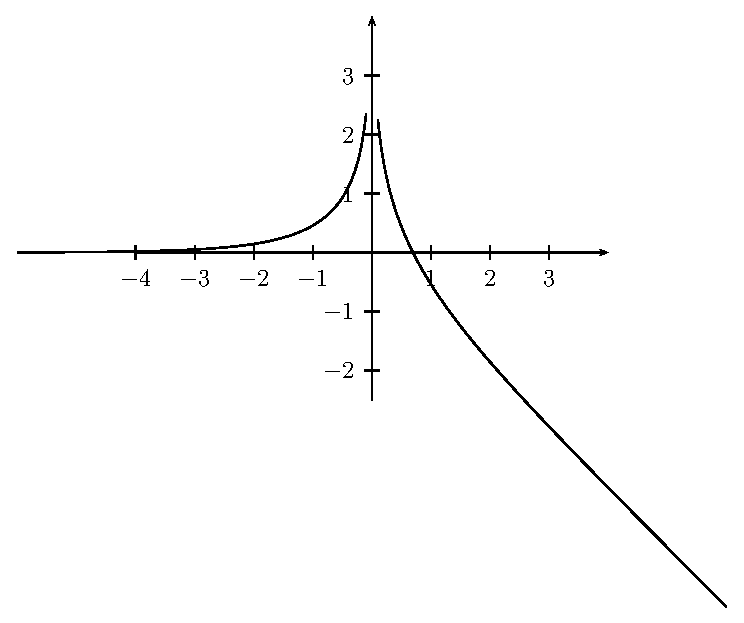
\includegraphics{../images/img005443-14}$$}
\end{enumerate}
}
